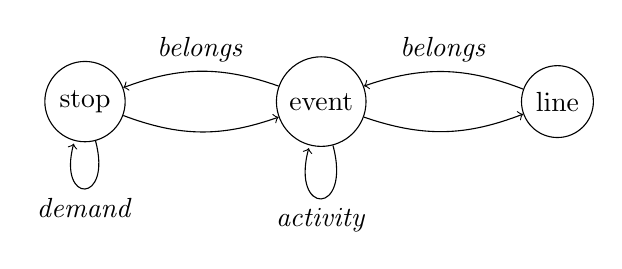
\begin{tikzpicture}[node distance=3cm, auto, swap]
    \tikzstyle{node}=[circle,draw]
    \node (event) [node] {event} edge [loop below] node {\textit{activity}} ();
    \node (stop) [node][left of=event] {stop} edge [loop below] node {\textit{demand}} ();
    \node (line) [node] [right of=event, node distance=3cm] {line};
    \draw [->] (stop) to [bend right=20] (event);
    \draw [->] (event) to [bend right=20] node {\textit{belongs}} (stop);
    \draw [->] (event) to [bend right=20] (line);
    \draw [->] (line) to [bend right=20] node {\textit{belongs}} (event);
    % \node {heimoi};
\end{tikzpicture}